\chapter{The Physics of Accretion}

\label{sec:PhysAcc}

\epigraph{\textit{A black hole consumes matter, sucks it in, and crushes it beyond existence. When I first heard that, I thought that's evil in its most pure.}}{Alice Morgan -- \textit{Luther}}

\vspace{1cm}

\par\noindent The extreme environments in accreting\index{Accretion} systems lead to a variety of somewhat unintuitive physical effects and phenomena.  In this chapter I describe a number of these effects, and delve into the history of physical and mathematical models which have been proposed to explain the effects seen in X-ray binaries.

\section{The Shakura-Sunyaev Disk Model}

\par\index{Shakura-Sunyaev disk model} To try and understand the behaviour of accretion disks\index{Accretion disk}, a number of authors have constructed models.  Much of our understanding of the physics of astrophysical accretion disks stems from one of the earliest of these models, proposed by Nikolai Shakura and Rashid Sunyaev in 1973 \citep{Shakura_Disk}.  This model specifically considered the effects of accretion\index{Accretion} onto a black hole\index{Black hole}.  By showing that this would result in a system which would be bright in the X-ray, and describing how such a system would appear, this model proved pivotal in the scientific community's acceptance of the earliest XRB identifications (e.g. \citealp{Bolton_CygX1}).
\par \citeauthor{Shakura_Disk} model the accretion disk\index{Accretion disk} as a structure held up by centrifugal forces, generated by the large amount of angular momentum\index{Angular momentum} possessed by infalling matter due to the orbit of the binary system.  Frictional forces cause this angular momentum to be transferred outwards, heating up the disk and allowing matter to fall in towards the black hole\index{Black hole}.  The efficiency with which this angular momentum is transferred can be thought of as a measure of the viscosity\index{Viscosity} of the disk.
\par \citeauthor{Shakura_Disk} base their calculations on Newtonian mechanics; as such they ignore the region of the disk\index{Accretion disk} inwards of the ISCO\index{Innermost stable circular orbit} at $r=3r_g$, where relativistic effects become important.  They also assume that the disk in a steady state, that it is geometrically thin (such that height of the disk $H\ll r$ everywhere) and that it is cylindrically symmetric.  The last two assumptions allow us to write down formulae for the surface density $\Sigma$, mean radial bulk velocity $u_r$ and accretion rate\index{Accretion rate} $\dot{M}$ of the disk as a functions of radius $r$:
\begin{eqnarray}
\Sigma(r)&=&\int_{-H}^H\rho(r,z) dz\label{eq:base1}\\\nonumber \\
u_r(r)&=&\frac{1}{\Sigma(r)}\int_{-H}^H\rho(r,z)v_r(r,z)dz\label{eq:base2}\\\nonumber \\
\dot{M}(r)&=&-2\pi r\Sigma(r) u_r(r)\label{eq:base3}
\end{eqnarray}
Where $\rho(r,z)$ is the density at a radius $r$ and height $z$, and $v_r$ is the radial velocity of the gas at this point.
\par Now consider the Euler equations of hydrodynamics:
\begin{eqnarray}
\frac{\partial\rho}{dt}+\dv(\rho\bm{v})&=&0\label{eq:consmass}\\\nonumber \\
\rho\left(\frac{\partial\bm{v}}{dt}+(\bm{v}\cdot\dv) \bm{v}\right)&=&-\dv p\label{eq:fma}
\end{eqnarray}
Where Equation \ref{eq:consmass} is the conservation of mass and Equation \ref{eq:fma} is a differential form of Newton's second law of motion.  These equations can be cast in cylindrical co-ordinates to give 4 equations: the recast continuity equation and one motion equation for each of the radial ($r$), vertical ($z$) and azimuthal ($\theta$) directions:
\begin{eqnarray}
\frac{\partial\rho}{\partial t}+\frac{1}{r}\frac{\partial(r\rho v_r)}{\partial r}+\frac{1}{r}\frac{\partial v_\theta}{\partial\theta}+\frac{\partial v_z}{\partial z}&=&0\label{eq:ssc}\\\nonumber\\
\rho\left(\frac{\partial v_r}{\partial t}+v_r\frac{\partial v_r}{\partial r}+\frac{v_\theta}{r}\frac{\partial v_r}{\partial\theta}+v_z\frac{\partial v_r}{\partial z}-\frac{v_\theta^2}{r}\right)&=&\frac{-\partial p}{\partial r}\label{eq:ssr}\\\nonumber\\
\rho\left(\frac{\partial v_\theta}{\partial t}+v_r\frac{\partial v_\theta}{\partial r}+\frac{v_\theta}{r}\frac{\partial v_\theta}{\partial\theta}+v_z\frac{\partial v_\theta}{\partial z}+\frac{v_rv_\theta}{r}\right)&=&\frac{-\partial p}{\partial\theta}\\\nonumber\\
\rho\left(\frac{\partial v_z}{\partial t}+v_r\frac{\partial v_z}{\partial r}+\frac{v_\theta}{r}\frac{\partial v_z}{\partial\theta}+v_z\frac{\partial v_z}{\partial z}\right)&=&\frac{-\partial p}{\partial z}\label{eq:ssz}
\end{eqnarray}
By assuming that the disk\index{Accretion disk} is in a steady state and cylindrically symmetric, we can set all $\frac{\partial}{\partial\theta}$ and $\frac{\partial}{\partial t}$ terms to zero, simplifying equations \ref{eq:ssr} to \ref{eq:ssz}:
\begin{eqnarray}
\rho\left(v_r\frac{\partial v_r}{\partial r}+v_z\frac{\partial v_r}{\partial z}-\frac{v_\theta^2}{r}\right)&=&\frac{-\partial p}{\partial r}\label{eq:ssrs}\\\nonumber\\
\rho\left(v_r\frac{\partial v_\theta}{\partial r}+v_z\frac{\partial v_\theta}{\partial z}+\frac{v_rv_\theta}{r}\right)&=&0\label{eq:ssts}\\\nonumber\\
\rho\left(v_r\frac{\partial v_z}{\partial r}+v_z\frac{\partial v_z}{\partial z}\right)&=&\frac{-\partial p}{\partial z}\label{eq:sszs}
\end{eqnarray}
We can average the density term on left-hand side of Equation \ref{eq:ssc} in the $z$-direction, and substitute in the results from Equations \ref{eq:base1} to \ref{eq:base3} to find:
\begin{eqnarray}
\frac{1}{r}\frac{d}{dr}\left(r\int_{-H}^H\rho v_rdz\right)&=&0\\\nonumber\\
\frac{1}{r}\frac{d(r\Sigma u_r)}{dr}&=&0\\\nonumber\\
\frac{-1}{2\pi r}\frac{d\dot{M}}{dr}&=&0
\end{eqnarray}
Therefore the rate of inwards matter flow $\dot{M}$, or the accretion rate\index{Accretion rate}, is constant at all $r$.
\par Using the fact that the angular velocity $\omega$ of an element in the gas can be written as $\omega=v_\theta/r$, we can re-write Equation \ref{eq:ssrs} as:
\begin{equation}
\rho\left(v_r\frac{\partial v_r}{\partial r}-\omega^2r\right)=-\frac{\partial p}{\partial r}-\rho v_z\frac{GM}{r^2}
\end{equation}
Where the term $\frac{GM}{r^2}$ has been introduced to account for the fact that the gradient of the gravitational field\index{Gravitational field} in the $r$ direction is non-zero.  This leads to:
%We can rewrite $v_z\frac{\partial v_r}{\partial z}$ as $\frac{\partial v_r}{\partial z}\frac{\partial z}{\partial t}$, which is equal to the inwards acceleration of a gas element moving in the $z$-direction.  As the disk is assumed to be in a cylindrically symmetric gravitational potential, this acceleration can be given by $\dot{v}_r=\frac{GM}{r^2}$.
\begin{equation}
\rho\left(v_r\frac{\partial v_r}{\partial r}-\omega^2r\right)=-\frac{\partial p}{\partial r}-\rho\omega_k^2r
\end{equation}
Assuming that is thin and angular momentum is only transferred slowly, i.e. $v_r\frac{\partial v_r}{\partial r}\ll\omega$, this leads to:
\begin{equation}
\omega\approx\omega_k
\end{equation}
Showing that gas elements in the disk\index{Accretion disk} orbit at Keplerian\index{Keplerian motion} speeds.
\par Using similar logic, Equation \ref{eq:sszs} becomes:
\begin{equation}
\rho\omega_k^2 z=\frac{-\partial p}{\partial z}\label{eq:idgas}
\end{equation}
The ideal gas law $p=\rho RT$\footnote{$R$ is the specific gas constant, equal to the Boltzmann Constant $k_B$ divided by the mean molar mass of the gas.} can then be used to rewrite equation \ref{eq:idgas}:
\begin{equation}
\frac{p}{RT}\omega_k^2 z=\frac{-\partial p}{\partial z}\label{eq:idgas2}
\end{equation}
If we assume that the disk\index{Accretion disk} is chemically homogeneous and isothermal in the $z$-direction, then neither $R$ nor $T$ depend on $z$.  Equation \ref{eq:idgas2} then admits the solution:
\begin{equation}
\rho=\rho_0(r)e^{\left(\frac{-z^2\omega_k^2}{2RT}\right)}=\rho_0(r)e^{\frac{-z^2}{2H_s^2}}
\end{equation}
Where $\rho_0$ is the density at radius $r$ when $z=0$.  As such, the density of the disk\index{Accretion disk} has a Gaussian profile in the $z$-direction, with a scale-width $H_s$ given by:
\begin{equation}
H_s=\frac{\sqrt{RT}}{\omega_k}
\end{equation}
This shows that the scale height of the disk\index{Accretion disk} is finite for all $r$.  As the integral between $-\infty$ and $+\infty$ of a Gaussian with a finite scale-width is finite, the disk contains a finite amount of matter.
\par Finally, \citeauthor{Shakura_Disk} looked at the solutions to Equation \ref{eq:ssts}.  As every term in this equation depends on either $v_\theta$ or a derivative thereof, this equation admits the solutions $\rho=0$ or $v_\theta=0$.  Both of these solutions imply accretion rates\index{Accretion rate} of zero, as any matter in the disk\index{Accretion disk} must have a non-zero density and angular momentum\index{Angular momentum}.  In order to resolve this problem, \citet{Shakura_Disk} add the divergence of the viscous stress tensor \citep{Landau_Tensor} to the right-hand side of Equation \ref{eq:ssts} to represent the effects of viscosity\index{Viscosity} within the disk\index{Accretion disk}.  By doing this, they find the following two results:
\begin{eqnarray}
\dot{M}&=&\frac{4\pi H_s\eta_b r}{\omega}\frac{\partial\omega}{\partial r}\label{eq:diffrot}\\\nonumber\\
\dot{M}&=&6\pi\eta_b H_s\label{eq:viscos}
\end{eqnarray}
Equation \ref{eq:diffrot} confirms that the disk\index{Accretion disk} is a differential rotator, while Equation \ref{eq:viscos} confirms that accretion\index{Accretion} can only take place when $\eta_b$ (the bulk viscocity) is non-zero.
\par \citet{Shakura_Disk} found that molecular viscosity\index{Viscosity} alone cannot be high enough to result in the high values of $\dot{M}$ inferred for observed XRBs.  Instead, the authors assume that turbulence\index{Turbulence} is present in the disk\index{Accretion disk}.  Using formulae pertaining to turbulent hydrodynamics, and by ignoring supersonic perturbations, they find an upper bound on bulk viscosity $\eta$:
\begin{equation}
\eta_b\leq\frac{2}{3}\rho_0H\sqrt{RT}
\end{equation}
As such, they define a dimensionless viscosity parameter $\alpha$ as:
\begin{equation}
\alpha\equiv\frac{3\eta_b}{2\rho_0H\sqrt{RT}}\quad\quad\quad0<\alpha\leq1
\end{equation}

\subsection{The source of Turbulence}

\par \citet{Shakura_Disk} do not answer the question of what physical process causes the turbulence\index{Turbulence} required to stabilise accretion disks\index{Accretion disk}.  \citet{Balbus_MRI} were among the first to propose the Magnetorotational Instability \citep[MRI,][]{Velikhov_MRI,Chandrasekhar_MRI}\index{Magnetorotational instability} as the source of this turbulence.  MRI\index{MRI|see {Magnetorotational instability}} is a process which occurs in an ionised and differentially rotating disk.  Fluctuations in the material in the disk generate internal magnetic fields\index{Magnetic field}.  The field lines associated with these fields, in general, extend a finite distance in the radial direction, thus connecting gas elements at different radii.  As gas elements in a Shakura-Sunyaev accretion disk\index{Shakura-Sunyaev disk model}\index{Accretion disk} orbit the compact object\index{Compact object} at Keplerian speeds\index{Keplerian motion}, elements of gas at different radii move at different orbital speeds.  As such, these internal magnetic field lines become stretched as gas orbits the compact object.  This field line stretching imparts a torque on the gas elements, causing the outer, slower element to speed up and the inner, faster element to slow down.  As such, the net result of this process is an outwards transfer of angular momentum\index{Angular momentum}.
\par \citet{Balbus_MRI} found that the angular momentum transfer due to MRI\index{Magnetorotational instability} was more significant than that due to friction, hydrodynamic turbulence\index{Turbulence} or other sources in an accretion disk\index{Accretion disk}.  They suggest therefore that MRI is the main component of outwards angular momentum\index{Angular momentum} transfer, and thus of $\alpha$\index{Viscosity}, in astrophysical accretion disks.

\section{Accretion Phenomena}

\par The extreme physics involved in accretion\index{Accretion} onto compact objects\index{Compact object} leads to a number of non-intuitive physical phenomena.  In this section I describe a number of these theoretical effects, and explain how these phenomena manifest in physical LMXBs.  

\subsection{The Eddington Limit}

\label{sec:edd}

\par\index{Eddington limit}\index{Eddington luminosity|see {Eddington limit}}\index{Eddington rate|see {Eddington limit}} Consider an element of gas at distance $r$ from a compact object\index{Compact object}, with mass $m$.  This element of gas is acted on by a inwards-pointing gravitational force given by:
\begin{equation}
F_G=\frac{GMm}{r^2}
\end{equation}
Where $M$ is the mass of the compact object.
\par If we assume that a luminosity $L$ is emitted isotropically from the compact object\index{Compact object}, then the electromagnetic flux at distance $r$ is given by:
\begin{equation}
\phi(r)=\frac{L}{4\pi r^2}
\end{equation}
Electromagnetic radiation exerts a pressure on material corresponding to $\phi/c$.  As such, the radiation from the X-ray binary exerts an outwards force on our gas element corresponding to:
\begin{equation}
F_L=\frac{\kappa m\phi(r)}{c}=\frac{L\kappa m}{4\pi r^2c}
\end{equation}
Where $\kappa$ is the opacity\index{Opacity} of the cloud, or its surface area per unit mass.
\par If $F_G$ and $F_L$ are equal, then no net force is exerted on our cloud of matter and it will not accrete\index{Accretion} onto the compact object\index{Compact object}.  This happens when:
\begin{eqnarray}
F_G&=&F_L\\ \nonumber \\
\frac{GMm}{r^2}&=&\frac{L\kappa m}{4\pi r^2c} \\ \nonumber \\
L&=&\frac{GMm}{r^2}\frac{4\pi r^2c}{\kappa m} \\ \nonumber \\
L&=&\frac{4\pi GMc}{\kappa}
\end{eqnarray}
This luminosity, denoted as $L_E$, is the Eddington luminosity; the theoretical maximum isotropic luminosity an object can emit and still have spherically symmetric accretion\index{Accretion} take place.  It only depends on the mass of the compact object\index{Compact object} $M$ and the opacity\index{Opacity} of the accreting\index{Accretion} material $\kappa$, which in turn depends on the chemical composition of the accretion disk\index{Accretion disk}.  As accretion disks tend to be dominated by ionised hydrogen, $\kappa$ is usually assumed to be $\sigma_T/m_p$, where $\sigma_T$ is the Thomson scattering cross-section\index{Thomson scattering cross-section} of an electron and $m_p$ is the mass of a proton.  This assumption yields the final formula which only depends on the mass of the compact object:
\begin{equation}
L_E=\frac{4\pi GMm_pc}{\sigma_T}
\end{equation}
The luminosity due to matter falling into a compact object\index{Compact object} can be expressed as:
\begin{equation}
L=\eta\dot{M}c^2
\end{equation}
Where $\dot{M}$ is the accretion rate\index{Accretion rate} and $\eta$ is the efficiency at which the gravitational potential energy of infalling matter is converted to outgoing radiation.  As such, $L_E$ also corresponds to a limiting accretion rate $\dot{M}_E$.
\par However, a number of X-ray binaries have been seen to shine at luminosities far above this limit; in one of the most extreme cases, the confirmed neutron star XRB M82 X-1 has a luminosity of $\sim100L_E$ \citep{Bachetti_M82X1}.  This super-Eddington\index{Super-Eddington accretion} accretion is possible due to the fact that a number of assumptions made when calculating the Eddington limit do not apply to physical XRBs.  In particular, the calculation performed above assumes that both accretion\index{Accretion} on to the compact object\index{Compact object}, as well as electromagnetic emission from it, are isotropic.  An object may exceed the Eddington Limit\index{Eddington limit} if it is accreting anisotropically, as is the case for XRBs\index{X-ray binary} as these systems accrete\index{Accretion} from near-planar disks\index{Accretion disk}.  In this case the assumptions behind the calculation of the Eddington Limit break down, and more radiation can be emitted away from the plane of the disk, decreasing the radiation pressure on infalling material.  Anisotropically emitting systems may appear to further exceed the Eddington limit via beaming effects.  An XRB beaming its radiation in the direction of the Earth would lead us to infer an artificially high value of $L$, and thus overestimate its luminosity with respect to the Eddington Limit.
\par Despite these setbacks, the Eddington Luminosity\index{Eddington limit} is a useful tool to compare XRBs\index{X-ray binary} with different compact object\index{Compact object} masses.  By expressing the luminosity of an object as a fraction of its Eddington Limit, objects can be rescaled in such a way that we can compare how dominant radiation pressure\index{Radiation pressure} must be in each accretion disk\index{Accretion disk}.

\subsection{The Propeller Effect}

\label{sec:prop}

\par\index{Propeller effect} Another limit on accretion rate\index{Accretion rate} arises when one considers the effect of a strong neutron star\index{Neutron star} magnetic field\index{Magnetic field}.  To understand this effect, we must first define two characteristic radii of such a system.
\par First, assume that the magnetic field\index{Magnetic field} of the neutron star\index{Neutron star} can be approximated as a set of rigid field lines which are anchored to points on the neutron star surface.  The magnetic field can then be thought of as a `cage' which rotates with the neutron star at its centre.  The straight-line speed of a point on this rotating cage is given by:
\begin{equation}
v_\nu(r)=2\pi r\nu
\end{equation}
Where $r$ is the distance from the neutron star centre and $\nu$ is the rotation frequency of the neutron star.  This can be compared with the Keplerian speed, or the speed of a particle in a Keplerian orbit\index{Keplerian motion} around the compact object\index{Compact object}.  This is given by:
\begin{equation}
v_K(r)=\sqrt{\frac{GM}{r}}
\end{equation}
Where $M$ is the mass of the neutron star.  By setting these equal, we can find the radius at which the magnetic field is rotating at the same speed as a particle in a Keplerian\index{Keplerian motion} orbit:
\begin{eqnarray}
v_\nu(r)&=&v_K(r)\\ \nonumber \\
2\pi r\nu&=&\sqrt{\frac{GM}{r}}\\ \nonumber \\
r^3&=&\frac{GM}{4\pi^2\nu^2}\\ \nonumber \\
r&=&\sqrt[3]{\frac{GM}{4\pi^2\nu^2}}
\end{eqnarray}
This radius is denoted as $r_c$, the co-rotation radius\index{Co-rotation radius}.  Inside of this radius, a particle in an equatorial Keplerian orbit\index{Keplerian motion} has a greater velocity than the magnetic field lines; outside this radius, the magnetic field lines are moving faster.  To understand the significance of this radius, we must define another characteristic radius of the system.
\par In a neutron star\index{Neutron star} accretion disk\index{Accretion disk}, there are three significant sources of pressure: gas (or ram) pressure\index{Ram pressure} $P_g$, radiation pressure $P_\gamma$\index{Radiation pressure} and magnetic pressure $P_\mu$\index{Magnetic pressure}.  Whichever pressure is dominant in a given location will govern the physics of matter in that region.
\par Photon pressure\index{Radiation pressure} falls off sharply outwards from the inner disk\index{Accretion disk}, so it can be assumed to be negligible in the region of the disk considered here.  We can then calculate where in the disk each of the remaining two pressures dominates.
\par Assuming that the neutron star behaves as a magnetic dipole, the magnetic pressure at a point a distance $r$ above its equator can be given as:
\begin{eqnarray}
P_\mu&=&\frac{B^2}{2\mu_0}\\ \nonumber \\
B(r)&=&B_0\left(\frac{R_{NS}}{r}\right)^3\label{eq:NS}\\ \nonumber \\
\therefore\quad P_\mu&=&\frac{B_0^2}{2\mu_0}\left(\frac{R_{NS}}{r}\right)^6
\end{eqnarray}
Where $\mu_0$ is the vacuum permeability, $B_0$ is the equatorial magnetic field strength at the neutron star surface, $R_{NS}$ is the radius of the neutron star and Equation \ref{eq:NS} is the equation for the magnetic field strength above the equator of a dipole.
\par The functional form of the ram pressure depends on the assumed accretion\index{Accretion} geometry of the system.  As when calculating the Eddington Limit, one can assume the simplest possible case of spherically accreting\index{Accretion} free-falling matter.  The ram pressure\index{Ram pressure} is then given by:
\begin{equation}
P_g=\frac{\dot{M}}{4\pi r^2}\sqrt{\frac{2GM}{r}}
\end{equation}
When $P_\mu>P_g$, accreting\index{Accretion} material is dominated by magnetic pressure\index{Magnetic pressure} in such a way that material is `frozen' onto magnetic field\index{Magnetic field} lines \citep{Alfven_Waves}; this results in material flowing onto the neutron star\index{Neutron star} surface along magnetic field lines onto the poles, as described in section \ref{sec:NSintro}.  It is possible to express the region of the accretion disk\index{Accretion disk} within which matter is magnetically dominated:
\begin{eqnarray}
P_g&<&P_\mu\\ \nonumber \\
\frac{\dot{M}}{4\pi r^2}\sqrt{\frac{2GM}{r}}&<&\frac{B_0^2}{2\mu_0}\left(\frac{R_{NS}}{r}\right)^6\\ \nonumber \\
\frac{GM\dot{M}^2}{8\pi^2 r^5}&<&\frac{B_0^4}{4\mu_0^2}\left(\frac{R_{NS}}{r}\right)^{12}\\ \nonumber \\
r^7&<&\frac{2\pi^2}{G\mu_0^2}\frac{B_0^4R_{NS}^{12}}{M\dot{M}^2}\\ \nonumber \\
r&<&\sqrt[7]{\frac{2\pi^2}{G\mu_0^2}\frac{B_0^4R_{NS}^{12}}{M\dot{M}^2}}\label{eq:rmu}
\end{eqnarray}
The critical radius, the magnetospheric or Alfv\'en radius\index{Magnetospheric radius}\index{Alfv\'{e}n radius|see {Magnetospheric radius}}, is denoted as $r_\mu$.
\par Now it is possible to consider what happens to matter approaching $r_\mu$ in two different physical regimes.  First of all, consider a system in which the corotation radius $r_c>r_\mu$.  In this case, which we show diagrammatically in panel A of Figure \ref{fig:propdiag}, magnetic field\index{Magnetic field} lines at $r_\mu$ are moving slower than the Keplerian speed\index{Keplerian motion}.  An element of matter approaching this radius from a Keplerian orbit will experience a torque slowing it down as it freezes onto the field lines.  This decrease in orbital speed causes the element's altitude above the neutron star surface to decrease.  This in turn pulls the element further into the magnetically-dominated regime and allows it to accrete\index{Accretion} freely along the field line onto the neutron star.

\begin{figure}
  \centering
  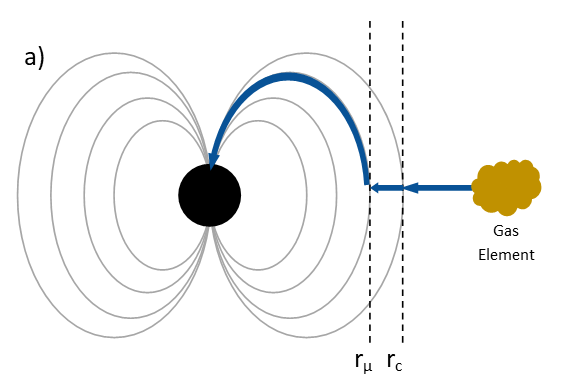
\includegraphics[width=0.7\linewidth, trim= 1mm 1mm 5mm 1mm, clip]{images/propeffd1.png}
  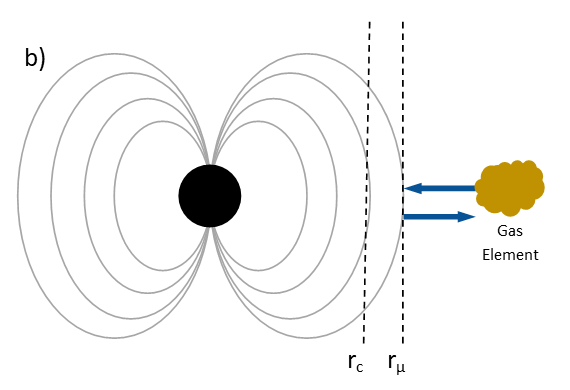
\includegraphics[width=0.7\linewidth, trim= 1mm 1mm 5mm 1mm, clip]{images/propeffd2.png}
  \caption[Diagrams showing the path of an element of gas in a neutron star accretion disk for different arrangements of the corotation and magnetospheric radii.]{Diagrams showing the path of an element of gas in a neutron star\index{Neutron star} accretion disk\index{Accretion disk} for different arrangements of the corotation\index{Co-rotation radius} ($r_c$) and magnetospheric\index{Magnetospheric radius} ($r_\mu$) radii.  In panel a), the gas falls freely inwards until it reaches $r_\mu$, at which point it freezes onto a magnetic field line.  As $r_\mu<r_c$, the magnetic field lines (grey lines) are rotating more slowly than the gas element at this point.  As such, the gas element experiences torque which slows it down, decreasing its altitude above the neutron star surface (black circle) and causing it to accrete\index{Accretion} along the magnetic field\index{Magnetic field} line.  In panel b), $r_\mu<r_c$.  As such, the magnetic field lines are rotating faster than the gas element at $r_\mu$.  The gas element experiences a torque which speeds it up at this point, increasing its altitude and preventing it from accreting\index{Accretion} onto the neutron star.}
  \label{fig:propdiag}
\end{figure}

\par Now we can consider what happens when $r_c<r_\mu$.  In this case, which we show diagrammatically in panel B of Figure \ref{fig:propdiag}, field lines at $r_\mu$ are moving faster than the Keplerian speed\index{Keplerian motion}.  An element of matter approaching $r_\mu$ will therefore experience a torque speeding it up as it becomes frozen onto magnetic field lines.  This will increase its altitude, driving it back away from $r_\mu$.  In this case, the magnetospheric radius acts as a barrier to infalling matter, repelling any gas that approaches it and stopping accretion\index{Accretion} onto the neutron star\index{Neutron star} surface.  This set of circumstances is known as the `propeller regime'\index{Propeller effect}, due to the rapidly rotating field\index{Magnetic field} lines acting like a `propeller' which blows the inner part of the disk\index{Accretion disk} away.
\par As the propeller\index{Propeller effect} regime is expected to occur only for $r_c<r_\mu$, it is possible to work out what kind of system this should be observed in:
\begin{eqnarray}
r_c&<&r_\mu\\ \nonumber \\
\left(\frac{GM}{4\pi^2\nu^2}\right)^{1/3}&<&\left(\frac{2\pi^2}{G\mu_0^2}\frac{B_0^4R_{NS}^{12}}{M\dot{M}^2}\right)^{1/7}\\ \nonumber \\
M^{10/21}\dot{M}^{2/7}&<&k\nu^{2/3}B_0^{4/7}R_{NS}^{12/7}\label{eq:ineq}
\end{eqnarray}
Where $k$ is a constant.  Assuming that the radius and mass of neutron stars does not vary much, this inequality tells us that the propeller regime is more likely to be observed in neutron star XRBs with a high spin frequency and a high magnetic field.  The inequality shown in \ref{eq:ineq} also tells us that the propeller effect places a \textit{lower} limit on accretion\index{Accretion} in such systems: accretion is not possible unless infalling matter can apply enough ram\index{Ram pressure} pressure to push the magnetospheric radius\index{Magnetospheric radius} inside the corotation\index{Co-rotation radius} radius.
\par There are numerous problems with this relatively simplistic view of accretion\index{Accretion} in a highly magnetic\index{Magnetic field} regime.  Much like the formulation of the Eddington Limit I present in Section \ref{sec:edd}, the above formulation of the propeller effect\index{Propeller effect} depends on an unphysical spherical accretion\index{Accretion} geometry.  It also includes the assumption that the magnetic field lines can in no way be warped by the movement of ionised matter on them.
\par \citet{White_MRad} have shown that, in neutron stars\index{Neutron star}, the magnetospheric radius\index{Magnetospheric radius} may be close enough to the compact object\index{Compact object} that photon pressure\index{Radiation pressure} cannot be safely neglected.  \citeauthor{White_MRad} find two different possible behaviours of the magnetospheric radius in such a regime, depending on how $\alpha$\index{Viscosity} varies with $r$ and how the disk\index{Accretion disk} reacts to the magnetic field\index{Magnetic field}.  For a perfectly diamagnetic disk, they show that the magnetospheric radius should not depend on the accretion rate\index{Accretion rate}, preventing the formation of a propeller regime\index{Propeller effect} entirely.  For a case in which gas pressure\index{Ram pressure} is the dominant contributor to viscous stress, they find that the magnetospheric radius is up to $\sim30$ times smaller than that calculated by equation \ref{eq:rmu}.  Additionally, \citet{Ertan_Prop} has analytically shown that an optically thick accretion disk can only be in a stable propeller regime when the inner disk radius is $\gtrsim15$ times smaller that the $r_\mu$ na\"ively calculated in equation \ref{eq:rmu}.  This in turn results in a several orders of magnitude reduction in the critical accretion rate at the onset of the propeller regime in a given system, raising questions as to whether the effect would be observable at such low luminosities.
\par Despite these difficulties, an effect observationally similar to the propeller effect is observed in a number of astrophysical neutron star XRBs (e.g. the cessation of pulsed emission while the source is still in outburst and the neutron star is actively spinning up or down, \citealp{Fabian_Propex,Furst_Propex}) and other systems (e.g. the observation of a sudden steepening in lightcurves during the decays of outbursts, interpreted by e.g. \citealp{Campana_PropBorder} as the onset of the propeller phase).  Therefore it is likely that a propeller effect in some form is likely able to explain what we see in nature.

\subsection{Disk Instabilities}

\label{sec:diskinstab}

\par\index{Instability}\index{Disk instability|see {Instability}} A number of effects can cause an accretion disk\index{Accretion disk}, or portions of it, to become unstable.  Some of these instabilities can set up limit cycles of behaviour in the disk, resulting in quasi-periodic fluctuations\index{Quasi-periodic oscillation}\index{QPO|see {Quasi-periodic oscillation}} in the object's intensity or colour\index{Colour} as seen from Earth.  I describe a number of these instabilities here.
\par One of the first such instabilities to be described was discovered by \citet{Lightman_Instability}.  Using the assumptions present in the thin disk\index{Accretion disk}\index{Shakura-Sunyaev disk model} models of \citet{Shakura_Disk} and \citet{Novikov_Torque}, \citeauthor{Lightman_Instability} calculate the diffusion\index{Diffusion} of the gas in such a disk.  They show that the diffusion coefficient in the radial direction of radiatively dominated disk is negative.  As such, any initially smooth disk under these conditions tends to separate into thin, dense annuli.  As such any sufficiently thin disk, with $\alpha$ consistent with the prescription of \citet{Shakura_Disk} is unstable.
\par \citet{Shakura_Instab} described another instability which takes place in the radiation pressure-dominated region near the inner edge of accretion disks\index{Accretion disk}.  They find that steady state accretion\index{Accretion} in such a regime is only possible for a single value of $\alpha$\index{Viscosity}, and hence this region is unstable under small perturbations of viscosity.  They argue that an instability\index{Instability} due to this effect may take the form of propagating wavefronts in the inner disk, which in turn may cause some of the quasiperiodic\index{Quasi-periodic oscillation} fluctuations which are observed in these objects.

\label{sec:hic}

\par A further disk\index{Accretion disk} instability\index{Instability} arises by considering the propeller effect\index{Propeller effect} (see Section \ref{sec:prop}), and specifically considering neutron star\index{Neutron star} LMXBs\index{X-ray binary!Low mass} in which the magnetopsheric radius\index{Magnetospheric radius} and co-rotation radius\index{Co-rotation radius} are similar ($r_c\approx r_\mu$, e.g. \citealp{Spruit_Type2Mod}).  At this boundary, a small increase in global accretion rate\index{Accretion rate} from the donor star pushes $r_\mu$ inwards such that $r_\mu<r_c$.  In this regime, the neutron star accretes freely, and the system is relatively bright in X-rays.  However, a slight decrease in global accretion rate causes $r_\mu<r_c$: in this regime, accretion\index{Accretion} onto the compact object\index{Compact object}'s surface is halted and the system is relatively faint in X-rays.  This effect causes a small fluctuation in accretion rate to convert to a large fluctuation in luminosity between two quasi-stable values.  This effect is believed to be behind the so-called `hiccup accretion'\index{Hiccup accretion} seen in X-ray binaries such as IGR J18245-2452\index{IGR J18245-2452} \citep{Ferrigno_TMSPVar} and 1RXS J154439.4-112820\index{3FGL J1544.6-1125} \citep{Bogdanov_Proxy}.

\section{GRS 1915+105 and IGR J17091-3624}

\label{sec:1915}

\par One famous system in which disk\index{Accretion disk} instabilities\index{Instability} are extremely apparent is the black hole\index{Black hole} LMXB\index{X-ray binary!Low mass} GRS 1915+105\index{GRS 1915+105}.  GRS 1915+105 \citep{CastroTirado_GRS1915}, hereafter GRS 1915, is a black hole LMXB\index{X-ray binary!Low mass} which accretes\index{Accretion} at between a few tens and more than 100\% of its Eddington Limit\index{Eddington limit} (e.g. \citealp{Vilhu_SupEd,Done_GRS_HighAcc,Fender_DiskJet}).  The system lies at a distance of $8.6\pm2.0$\,kpc \citep{Reid_Parallax}, and consists of a 12.4$\pm$2.0\,M$_\odot$ black hole\index{Black hole} and a $<1$\,M$_\odot$ K-class giant companion star\index{Companion star} \citep{Reid_Parallax,Ziolkowski_GRSDonor}.
\par The components of GRS 1915 have the longest known orbital period\index{Orbital period} of any LMXB \citep{Greiner_BigDisk}, in turn implying that this system has the greatest orbital separation and the largest accretion disk\index{Accretion disk}.  GRS 1915 has been in outburst\index{Outburst} since its discovery in 1992 \citep{CastroTirado_GRS1915}, and the extreme length of this ongoing outburst is believed to be related to the large size of its accretion disk. 
\par GRS 1915 is also notable for the incredible variety and complexity of behaviours\index{Variability} it exhibits over timescales of seconds to minutes (e.g. \citealp{Yadav_GRSBursts,Belloni_GRS_MI}).  In total, at least 15 distinct `variability classes'\index{Variability class} have been described \citep{Belloni_GRS_MI,KleinWolt_OmegaClass,Hannikainen_NewClass, Pahari_NewClass}, a number of which I show lightcurves\index{Lightcurve}\footnote{A plot showing how the intensity of an object varies over time.} of in Figure \ref{fig:GRSsample}.  The system tends to stay in one variability class for no more than a few days but similar patterns are often repeated many months or years later, suggesting some capacity of the system to `remember' which variability classes it can show.

\begin{figure}
  \centering
  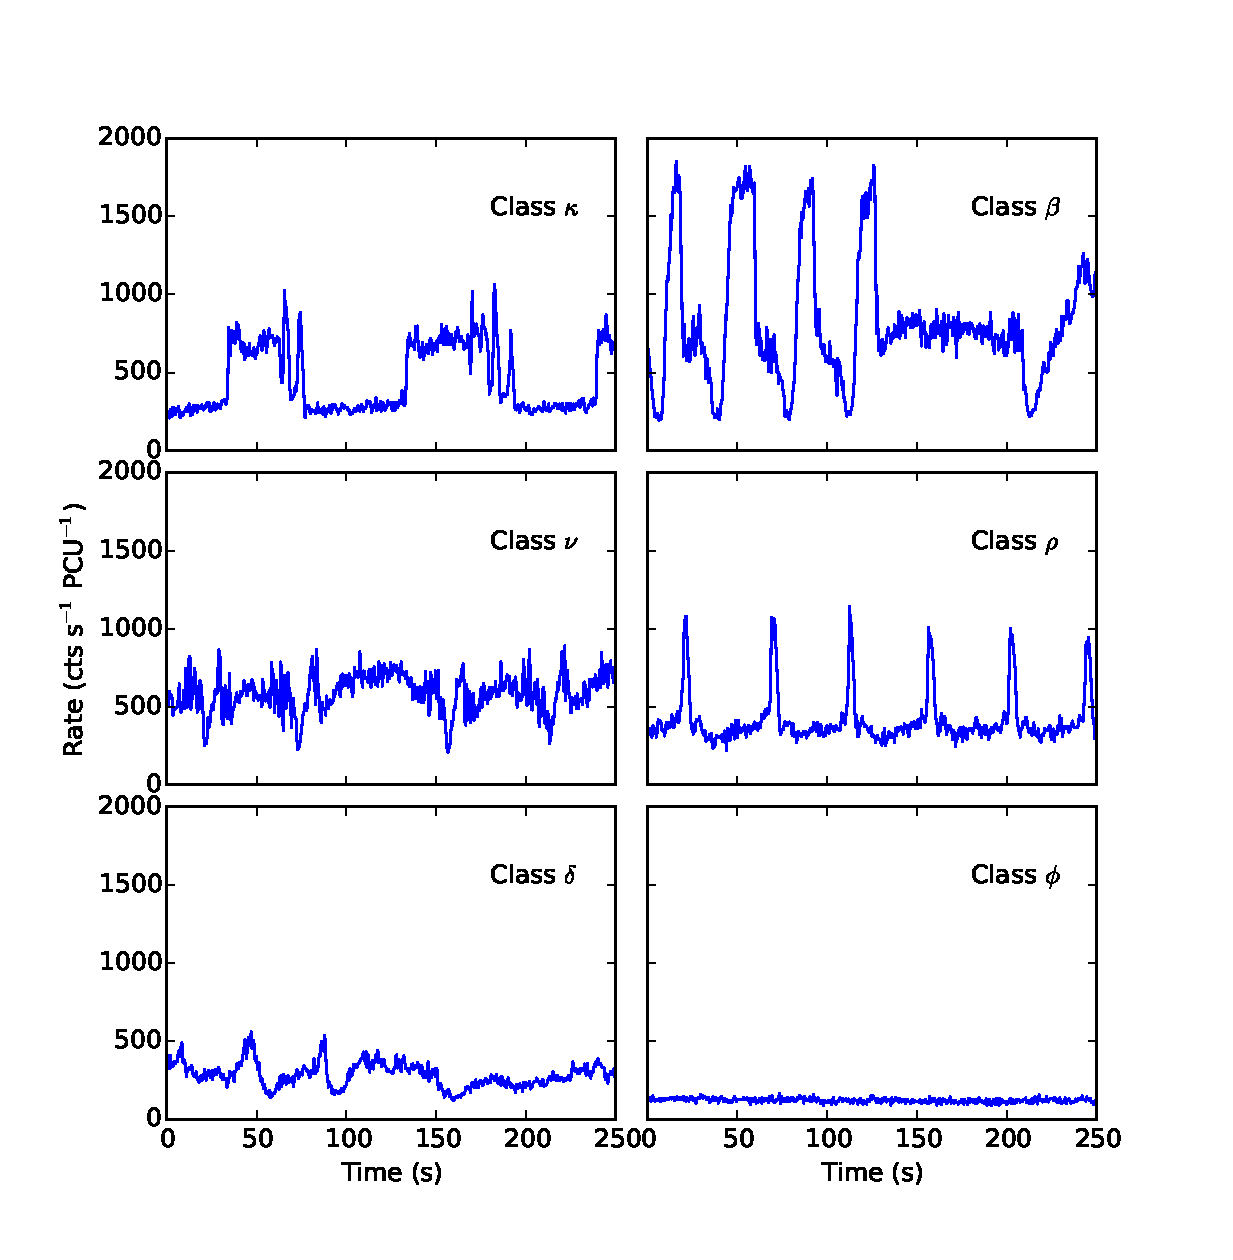
\includegraphics[width=\linewidth, trim= 0mm 0mm 0mm 0mm, clip]{images/GRSsample.eps}
  \caption[Typical lightcurves of a selection of variability classes seen in the LMXB GRS 1915+105.]{\indexkappa\indexnu\indexbeta\indexrho\indexdelta\indexphi Typical lightcurves\index{Lightcurve} of a selection of variability classes\index{Variability class} seen in GRS 1915, taken by the PCA instrument aboard \rxte\indexrxte\indexpca.  The classes are labelled according to the Greek letter names assigned to them in \citet{Belloni_GRS_MI}.}
  \label{fig:GRSsample}
\end{figure}

\par The variability classes of GRS 1915 consist of repeating patterns of flares\index{Flare}, dips\index{Dip} and periods of noisy fluctuation, with a range of amplitudes and timescales.  The  behaviour of the source during these classes, which are usually denoted by the Greek letter names assigned to them by \citet{Belloni_GRS_MI}, can range from highly quasi-periodic to apparently entirely unstructured.  The $\rho$\indexrho\ class, also referred to as the `heartbeat'\index{Heartbeat|see {Variability class, $\rho$}} class due to the similarity of its lightcurve to the output of an electrocardiagram, consists of sharp quasiperiodic flares\index{Quasi-periodic oscillation} with a recurrence time\index{Recurrence time} of a few tens of seconds (Middle-right panel of Figure \ref{fig:GRSsample}).  Other classes, such as class $\kappa$\indexkappa\ shown in the top-left panel of Figure \ref{fig:GRSsample}, consist of quasiperiodic fluctuations between two quasistable count rates: in the case of class $\kappa$, there is also a period of highly structured sub-second variability at each transition between these two classes.  Finally, two classes ($\chi$\indexchi\ and $\phi$\indexphi, an example of the latter is shown in the bottom-right panel of Figure \ref{fig:GRSsample}) show no significant variability other than red noise; these classes are separated from each other based on their spectral properties.  It has been suggested they they may be equivalent to the hard state\index{Low/Hard state} seen in other outbursting LMXBs \citep{VanOers_GRSHard}, providing a possible link between the behaviour of GRS 1915 and the behaviour of more typical LMXBs.
\par The dramatic variability seen in GRS 1915\index{GRS 1915+105} was long thought to be unique, driven by its unusually high accretion rate\index{Accretion rate} (e.g. \citealp{Belloni_Timescales}).  However in 2011, \citet{Altamirano_IGR_FH} unambiguously identified GRS 1915-like variability in a second object: the black hole\index{Black hole} LMXB\index{X-ray binary!Low mass} IGR J17091-3624\index{IGR J17091-3624} (hereafter IGR J17091).  This object is much fainter than GRS 1915: \citet{Altamirano_IGR_FH} showed that, assuming that this object accretes\index{Accretion} at its Eddington Limit\index{Eddington limit} by analogy with GRS 1915, the object may either be out in the halo of the Galaxy (at $\gtrsim20$\,kpc) or harbour the smallest mass black hole known to science ($\lesssim3$\,M$_\odot$).  The companion star\index{Companion star} to the black hole in this system has not been definitively identified \citep{Chaty_IGRCompanion}.
\par Much like GRS 1915\index{GRS 1915+105}, IGR J17091\index{IGR J17091-3624} displays a number of distinct classes of variability\index{Variability class} over time, and a number of these have been identified as being similar to the classes seen in GRS 1915 (e.g. \citealp{Altamirano_IGR_FH,Zhang_IGR}).  Unlike GRS 1915, IGR J17091 displays the pattern of outbursts\index{Outburst} and quiescence\index{Quiescence} more commonly seen in LMXBs; known outbursts of IGR J17091 occurred in 2011 and 2016, and GRS 1915-like\index{Variability} variability was observed in both \citep{Reynolds_2016HB}.
\par There are a number of notable differences between variability classes in GRS 1915 and IGR J17091.  In general, variability classes in IGR J17091 occur over shorter timescales than their counterparts in GRS 1915.  In addition to this, hard emission\index{Hard lag} tends to lag soft emission in the variability classes of GRS 1915 (e.g. \citealp{Janiuk_Lag}), while the opposite trend has been found in the `heartbeat'-like\indexrho\ class of IGR J17091 \citep{Altamirano_IGR_FH}.
\par In addition to GRS 1915 and IGR J17091\index{IGR J17091-3624}, there have been claims that a third LMXB\index{X-ray binary!Low mass} displays GRS 1915\index{GRS 1915+105}-like variability\index{Variability}.  \citet{Bagnoli_RB} report on two observations of MXB 1730-335\index{MXB 1730-335|see {Rapid Burster}}, also known as the `Rapid Burster'\index{Rapid Burster}, which show lightcurve patterns remarkably similar to those seen in the $\rho$\indexrho\ and $\theta$\indextheta\ classes of GRS 1915.  The presence of GRS 1915-like variability in the Rapid Burster is significant for a number of reasons: unlike GRS 1915\index{GRS 1915+105} or IGR J17091\index{IGR J17091-3624}, the Rapid Burster is known to contain a neutron star\index{Neutron star} accreting\index{Accretion} at no more than 20\% of its Eddington Limit\index{Eddington limit}, thereby ruling out any black hole\index{Black hole}-specific or near-Eddington-specific explanations for this behaviour.  In addition to this, the Rapid Burster is one of only 2 objects known to undergo so-called Type II X-Ray bursts\index{X-ray burst!Type II} (see Section \ref{sec:TypeII}), suggesting a possible link between these two phenomena.  However, as it has only been observed twice in the $\sim30$ years since the object was discovered, the true nature of the apparent GRS 1915-like variability in the Rapid Burster remains unclear.

\subsection{A History of Models of GRS 1915-like Variability}

\label{sec:models_GRS}

\par Over the years, a number of models and physical scenarios have been suggested to explain the complex variability seen in GRS 1915-like\index{GRS 1915+105} systems.  Successful models must also be able to explain why this type of variability is not seen in a wider array of sources.
\par One of the most best-studied classes of GRS 1915-like variability is Class $\rho$\indexrho, the `heartbeat' class.  This variability class is present in both GRS 1915 and IGR J17091\index{IGR J17091-3624} (e.g. \citealp{Altamirano_IGR_FH}), and has been the focus of many of the models proposed to explain GRS 1915-like variability.  It has been shown that hard X-ray photons lag soft X-ray photons\index{Hard lag} in this class (e.g. \citealp{Janiuk_Lag,Massaro_Lag}), suggesting that hard emission from this source is somehow caused by the softer emission.  Other classes in GRS 1915 which show quasi-periodic flaring behaviour also exhibit this phase lag.  Previous authors have established models to explain both the hard photon lag as well as the `heartbeat'-like flaring itself, generally based on the instability\index{Instability} in a radiation-dominated disk\index{Accretion disk} first formulated by \citet{Shakura_Instab} (see Section \ref{sec:diskinstab}).
\par \citet{Belloni_Model1} first proposed an empirical model for flaring\index{Flare} in GRS 1915.  They suggested that this behaviour is due to a rapid emptying of a portion of the inner accretion disk\index{Accretion disk}, followed by a slower refilling of this region over a viscous timescale.  \citeauthor{Belloni_Model1} divided data from a given observation into equal-sized 2-Dimensional bins in count rate-colour\index{Colour} space.  A spectral\index{Spectroscopy} model was then fit to each of these bins independently to perform `pseudo'-phase-resolved spectroscopy\index{Spectroscopy!Phase-resolved} (compare with the method outlined in Section \ref{sec:phasresspec}).  They showed that the time between flaring\index{Flare} events correlates with the maximum inner disk radius during the flare; i.e., a correlation between the amount of the disk which is emptied and the time needed to refill it.  They go on to suggest that their model is able to explain all flaring-type events seen in GRS 1915.
\par The scenario proposed by \citet{Belloni_Model1} was mathematically formalised by \citet{Nayakshin_GRSModel}, who found that it was not consistent with a `slim' accretion disk\index{Accretion disk} \citep{Abramowicz_Slim} or with a disk in which viscosity $\alpha$\index{Viscosity}\index{Alpha@$\alpha$|see {Viscosity}} is constant with respect to radius.  As such, their model consists of a cold accretion disk with a modified viscosity law, a non-thermal electron corona\index{Corona} and a transient jet\index{Jet} of discrete plasma emissions which are ejected when the bolometric luminosity approaches the Eddington Limit\index{Eddington limit}.  Using their model, \citet{Nayakshin_GRSModel} found that some formulations of $\alpha(r)$\index{Viscosity} result in the disk oscillating between two quasi-stable branches in viscosity-temperature space, over timescales consistent with those seen in the flaring of GRS 1915; they found that this occurs for accretion rates\index{Accretion rate} greater than 26\% of the Eddington limit\index{Eddington limit}.  They also found that by varying the functional form of $\alpha(r)$\index{Viscosity}, their model gives rise to a number of lightcurve morphologies which generally match what is seen in data from GRS 1915.  \citet{Janiuk_RadInstab} built on this model further by including the effect of the transient jet\index{Jet} in cooling the disk; an effect not considered in the model by \citet{Nayakshin_GRSModel}.  In this formulation, \citet{Janiuk_RadInstab} found that GRS 1915-like variability should occur at luminosities as low as 16\% of Eddington.  The criteria of a relatively low accretion rate\index{Accretion rate} in these models suggests that many more black hole\index{Black hole} LMXBs should show GRS 1915-like behaviour, which is at odds with observations.  Additionally, they are unable to explain GRS 1915-like behaviour in objects with even lower accretion rates, such as the $\rho$-like\indexrho\ behaviour reported by \citet{Bagnoli_RB} in the Rapid Burster\index{Rapid Burster}.
\par \citet{Belloni_GRS_MI} found that variability in GRS 1915 can be empirically described by transitions between three phenomenological states, which differ in luminosity and hardness ratio:
\begin{enumerate}
\item State B: high rate, high 5--13/2--5\,keV hardness ratio.
\item State C: low rate, low 5--13/2--5\,keV hardness ratio, variable 13--60/2--5\,keV hardness ratio.
\item State A: low rate, low 5--13/2--5\,keV hardness ratio, lowest 13--60/2--5\,keV hardness ratio.
\end{enumerate}
\citeauthor{Belloni_GRS_MI} find that no variability class shows a transition from state C to state B, and they suggest that this transition is forbidden.  The phenomenological scenario they establish is at odds with the model of \citet{Nayakshin_GRSModel}, which only results in two quasi-stable states; one high rate and one low rate state.
\par \citet{Nobili_Hotspot} tried to account for the hard X-Ray lag\index{Hard lag} by considering a scenario in which a significant proportion of the X-Ray disk\index{Accretion disk} variability comes from a single hotspot.  They suggest that the lag corresponds to a light travel time, after which a portion of this emission is Comptonised\index{Compton scattering} by the jet.  In this case, the geometric location of this hotspot determines the magnitude of this lag.  This scenario goes some way to explaining why GRS 1915 is special, as it requires the presence of a jet\index{Jet} during a soft-like\index{High/Soft state} state.
\par \citet{Tagger_MagneticFlood} propose a magnetic explanation for the ejection of the inner accretion disk\index{Accretion disk} required by \citet{Nayakshin_GRSModel} and \citet{Janiuk_RadInstab}.  In their scenario, they suggest the existence of a limit cycle in which a poloidal magnetic field\index{Magnetic field} is advected towards the inner disk during the refilling of this region.  Associated field lines are then destroyed in reconnection\index{Reconnection} events, releasing energy which results in the expulsion of matter from the inner disk.  They suggest that the three quasi-stable states proposed by \citealp{Belloni_GRS_MI} can be explained as states in the inner accretion disk with different values of plasma $\beta$\index{Plasma $\beta$}\footnote{The ratio of the plasma pressure to the magnetic pressure in an ionised medium.}.
\par \citealp{Janiuk_Lag} attempt to explain the hard lag in the heartbeats\indexrho\ of GRS 1915\index{GRS 1915+105} more simply, by proposing a model in which it is caused by the non-thermal corona\index{Corona} smoothly adjusting to changes in luminosity from the disk\index{Accretion disk}.  They base the variability\index{Variability} of the disk on the model of \citealp{Nayakshin_GRSModel}, and show that the presence of a non-thermal corona which reacts to this variability naturally reproduces the lag behaviour seen in Class $\rho$\indexrho\ in GRS 1915.
\par \citealp{Merloni_MagDom} also propose a magnetic explanation for the reformulation of $\alpha(r)$ required by the model of \citealp{Nayakshin_GRSModel}.  Assuming that the viscosity in the accretion disk\index{Accretion disk} is dominated by turbulence\index{Turbulence} due to the magnetorotational instability\index{Magnetorotational instability}, they find that allowing for a magnetically dominated corona naturally allows for the forms of $\alpha(r)$ required by \citealp{Nayakshin_GRSModel}.
\par \citealp{Zheng_Model} propose a model which suggests that, when the effects of a magnetic field are included, the accretion rate\index{Accretion rate} threshold for GRS 1915-like\index{GRS 1915+105} variability\index{Variability} should be $\sim50$\% of Eddington\index{Eddington limit}; significantly higher than the 16\% or 26\% reported by \citealp{Janiuk_RadInstab} or \citealp{Nayakshin_GRSModel}.  \citeauthor{Zheng_Model} go on to suggest that this type of variability is only seen in GRS 1915 due to this source having the highest accretion rate\index{Accretion rate} of all permanently soft-state sources.  As such, this scenario still relies on a high accretion rate to trigger GRS 1915-like variability, but it is more consistent with observations than the models of \citealp{Janiuk_RadInstab} or \citealp{Nayakshin_GRSModel}.%  However, magnetohydronamic simulations of a radiation dominated inner disk performed by \citealp{Hirose_Stable} suggest that the thermal instabilities required by models of heartbeat should not arise at any value of accretion rate.
%\par \citealp{Xue_Spin} derive a mathematical model of the evolution of a slim accretion disk around a Kerr black hole.  They hypothesize that the spin of the black hole, not the accretion rate, may be the driving factor behind GRS 1915-variability.  However, they find that that the morphology of X-ray lightcurves from such a disk only has a weak dependence on the spin of the black hole, ruling this out as a possible explanation.

\label{sec:Neilsen}

\par \citealp{Neilsen_GRSModel} performed phase-resolved spectroscopy of the $\rho$\indexrho\ class in GRS 1915\index{GRS 1915+105}.  They find a hard `spike' after each flare, which they associate with the hard lag\index{Hard lag} in this class previously noted by e.g. \citealp{Janiuk_Lag}.  They propose a scenario in which high-velocity winds\index{Wind} formed by the ejection of matter from the inner disk\index{Accretion disk} interact directly with the corona\index{Corona} after a light travel time.  The corona then re-releases this energy as a hard bremsstrahlung pulse, causing the hard count rate spike seen in phase-resolved spectra.  This scenario is outlined in Figure \ref{fig:WindsModel}.  The authors expand on this scenario in \citealp{Neilsen_Rho} to suggest that this mechanism can explain all classes in GRS 1915 which display $\rho$-like flaring\index{Flare}.  However, this scenario still relies on the model of \citealp{Nayakshin_GRSModel} to generate the instability in the disk, and it implies that hard photons should always lag soft photons\index{Hard lag} in heartbeat-like variability classes.  Significantly, this scenario is therefore unable to explain the soft lags which have been observed in $\rho$-like variability in IGR J17091 \citep{Altamirano_IGR_FH}.

%\pagebreak
\begin{figure}
  \centering
  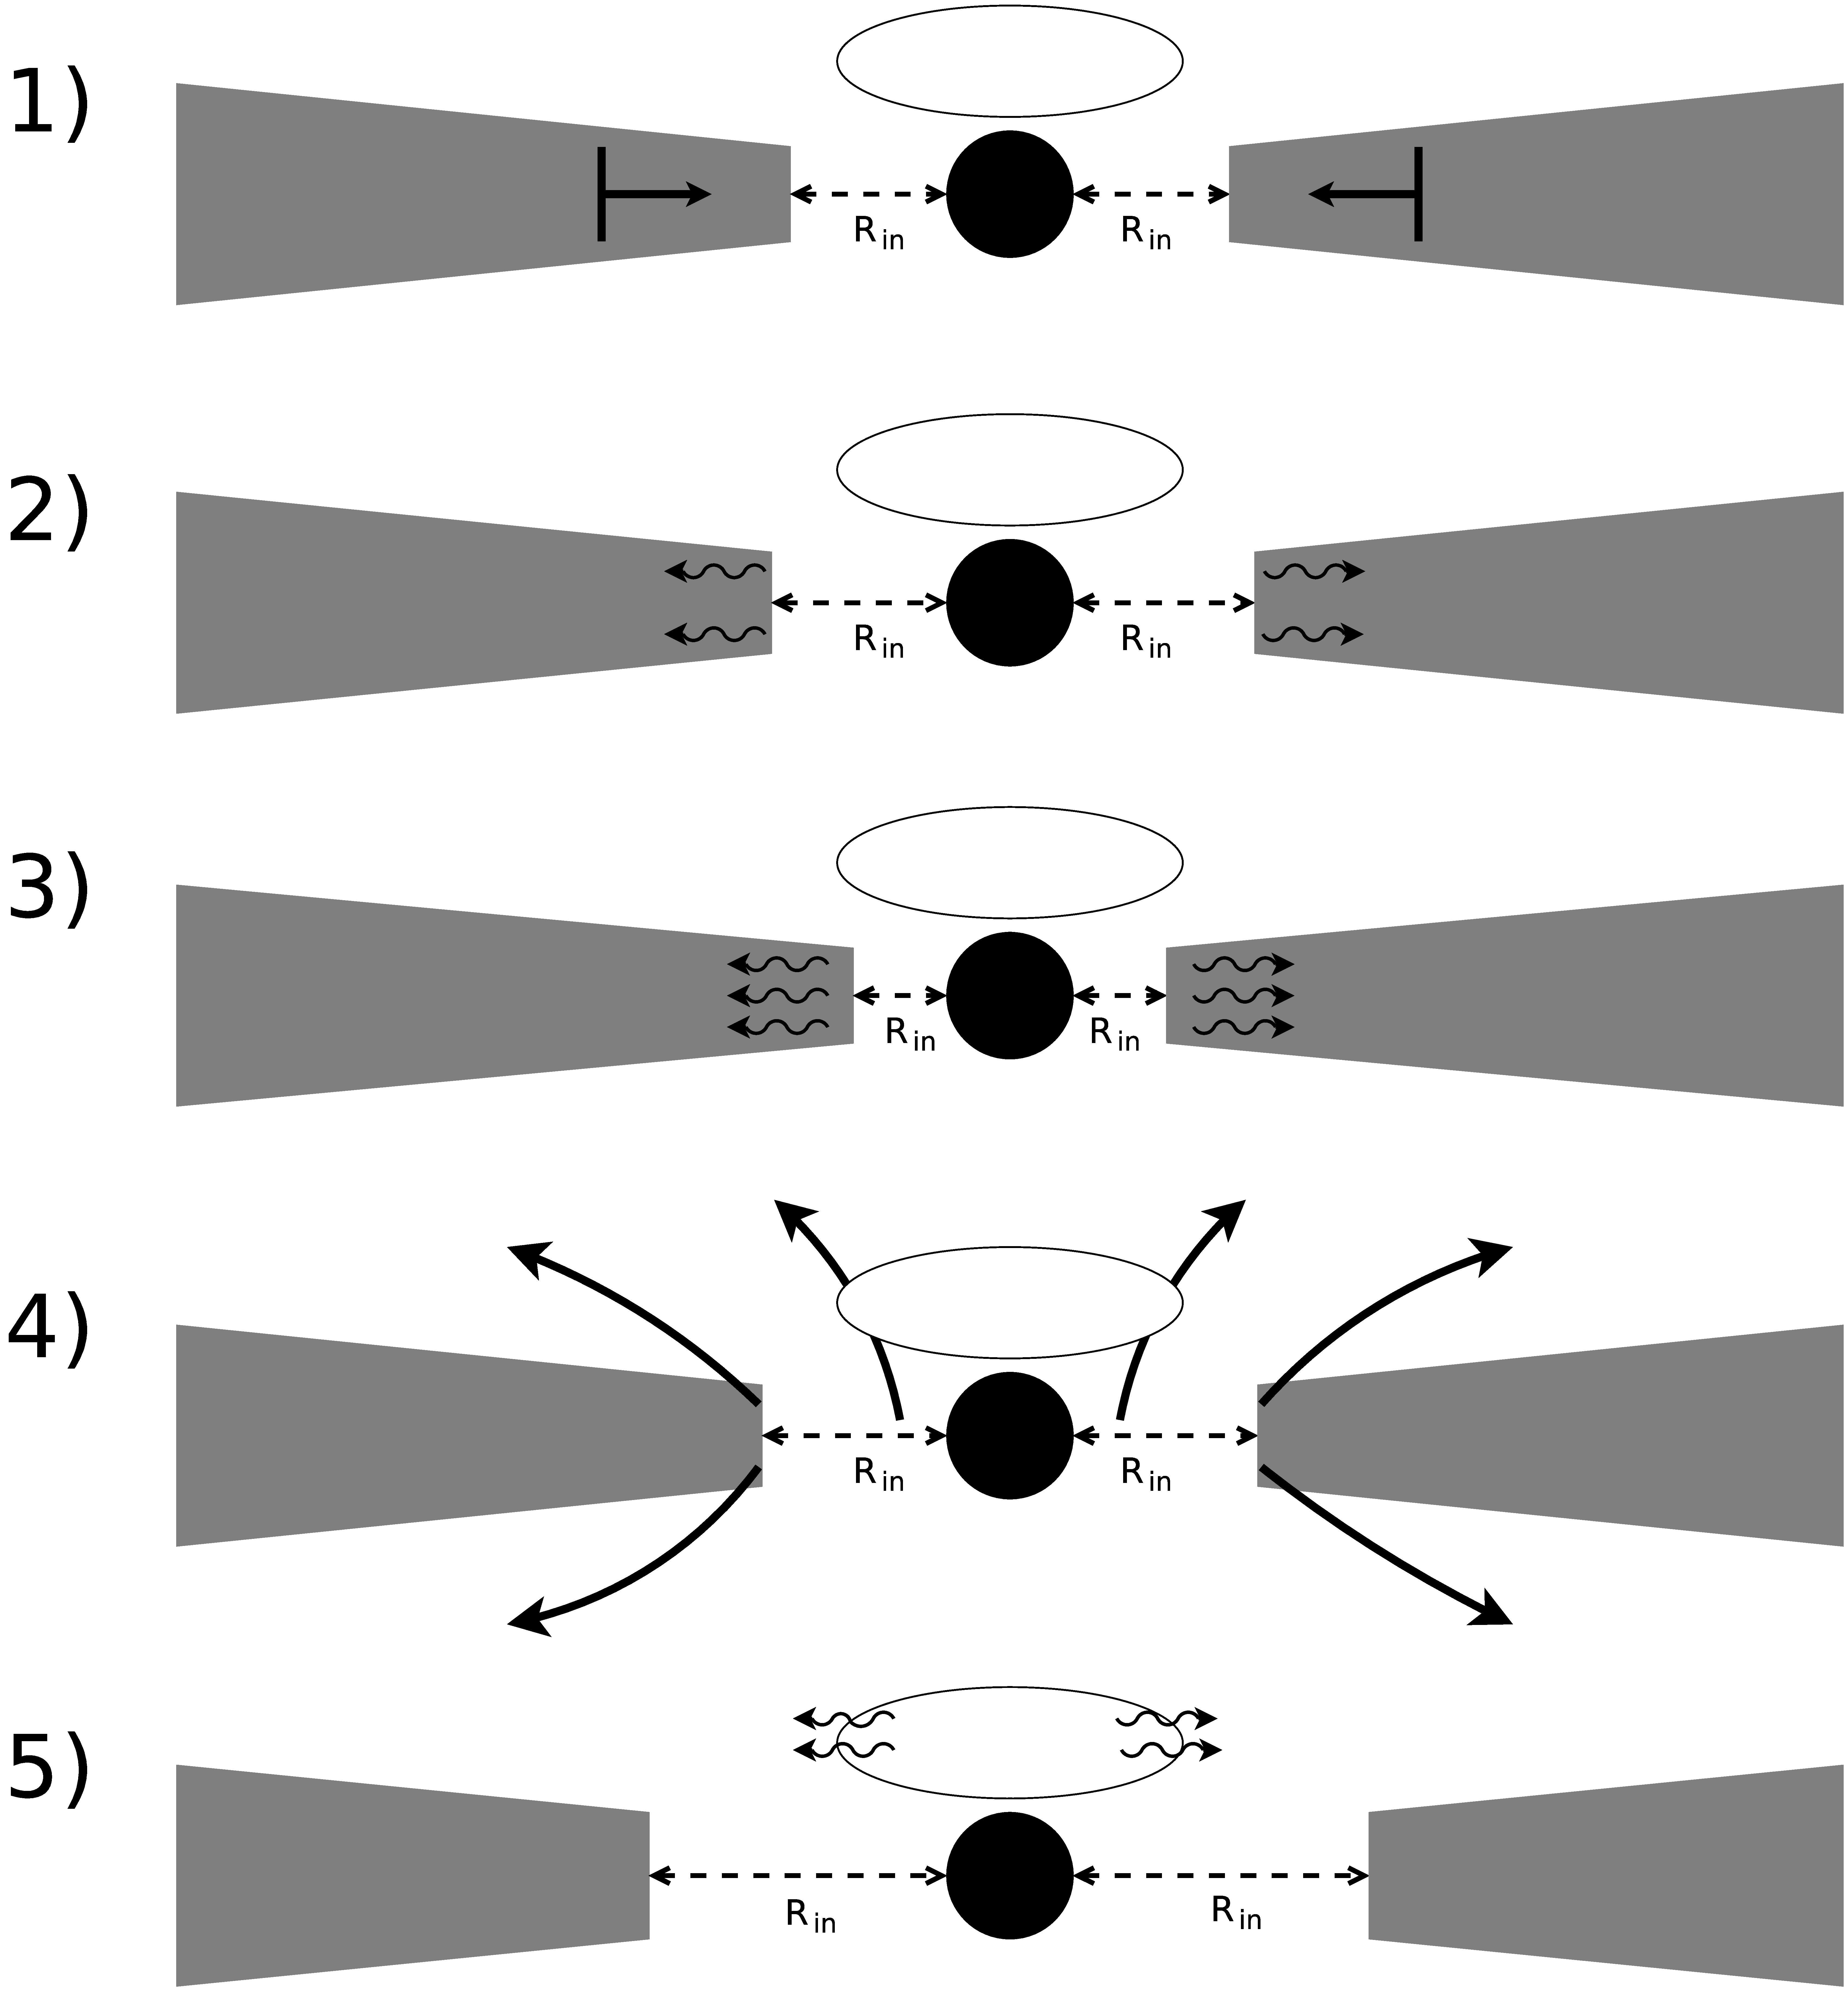
\includegraphics[width=.9\linewidth, trim= 25mm 0mm 0mm 0mm]{images/Wind_Model1.eps}
  \caption[A schematic diagram illustrating the the process described by \citet{Neilsen_GRSModel} to describe the $\rho$ variability class in GRS 1915+105.]{A schematic diagram illustrating the the process described by \citealp{Neilsen_GRSModel} to describe the $\rho$\indexrho\ variability class in GRS 1915+105\index{GRS 1915+105}.  1) The X-ray emission from the system originates from both the accretion disk\index{Accretion disk} truncated at an inner radius $r_{in}$ (grey) and a corona of non-thermal electrons\index{Corona} (white ellipse).  At some time $t$, an overdensity in the accretion disk\index{Accretion disk} (formed by the instability\index{Instability} described by \citealp{Shakura_Instab}) propagates inwards towards $r_{in}$.  2) As the inner disc heats up, $r_{in}$ begins to slowly increase due to an increase in photon pressure\index{Radiation pressure}.  This destabilises\index{Instability} the disc.  3) At some critical density, the disc becomes too unstable and collapses inwards, greatly decreasing $r_{in}$ and raising the inner disc temperature.  4) The sudden increase in emission exceeds the local Eddington limit\index{Eddington limit} at $r_{in}$, ejecting matter from the inner accretion disc in the form of extreme winds\index{Wind}.  5) Having been excited by matter in the winds passing through it, the non-thermal electron cloud emits a hard Brehmsstrahlung `pulse'.}
  \label{fig:WindsModel}
\end{figure}
%\pagebreak

\par \citealp{Neilsen_GRSModel} also perform phase-resolved spectroscopy\index{Spectroscopy!Phase-resolved} (see Section \ref{sec:phasresspec}) of the flaring during $\rho$ variability.  In their fitting, \citealp{Neilsen_GRSModel} consider three spectral models:
\begin{enumerate}
\item An absorbed disk black body with a high energy cutoff, of which some fraction has been Compton upscattered
\item An absorbed disk black body with a high energy cutoff, plus a Compton component with a seed photon spectrum tied to the emission from the disk
\item An absorbed disk black body plus a Compton component with a seed photon spectrum tied to the emission from the disk and a bremsstrahlung component
\end{enumerate}
They find that the first of these models (Model 1) is the best fit to the data.
\par \citealp{Mineo_PhasRes} also performed psuedo-phase-resolved spectroscopy\index{Spectroscopy!Phase-resolved} of the $\rho$\indexrho\ class in GRS 1915, using a number of different spectral models to \citealp{Neilsen_GRSModel} but a significantly lower phase resolution.  In this work, the authors consider six models:
\begin{enumerate}
\item A multi-temperature disk black body plus a corona containing both thermal and non-thermal electrons (as formulated by \citealp{Poutanen_Hybrid}).
\item A multi-temperature disk black body plus a multi-temperature disk black body plus a power law.
\item A multi-temperature disk black body plus an independent Compton component.
\item A multi-temperature disk black body plus a power law plus reflection from the outer disk.
\item A model of Comptonization due to the bulk-motion of matter in the disk.
\item A multi-temperature disk black body plus a power law plus a standard black body.
\end{enumerate}
With the exception of Models 1 and 6, the authors find that none of these models are able to satisfactorily fit the data in each of their phase bins independently.  As there is no reasonable physical explanation behind Model 6, the authors only consider Model 1.  Their results suggest a large reduction of the corona luminosity during each heartbeat flare, which they interpret as the corona\index{Corona} condensing onto the disk\index{Accretion disk}.  They also find that their results are consistent with GRS 1915\index{GRS 1915+105} having a slim disk, but inconsistent with the hard lag\index{Hard lag} being caused by photon upscattering in the corona.
\par \citealp{Massa_MoveLag} found that the magnitude of the lag\index{Hard lag} between hard and soft photons in the $\rho$-class\indexrho\ of GRS 1915\index{GRS 1915+105} is not constant.  They found that the lag varies between $\sim3$--$10$\,s, and correlates strongly with count rate.  The magnitude of the lag, therefore, is too large to be simply due to a light travel time to the corona\index{Corona} from the disk\index{Accretion disk}.  The authors suggest that their results are instead consistent with the thermal adjustment of the inner disk itself as part of the instability limit cycle invoked to explain the flares\index{Flare}.
\par \citealp{Massaro_Numerical} constructed a set of differential equations to mathematically model the behaviour of the oscillator underlying $\rho$-like flaring in GRS 1915.  They find that a change between variability classes likely corresponds to a a change in global accretion rate\index{Accretion rate}, but that the global accretion rate within the $\rho$ class is constant.  This model reproduces the count rate-lag correlation reported by \citealp{Massa_MoveLag}, as well as a previously reported correlation between flare recurrence time\index{Recurrence time} and count rate \citep{Massaro_Lag}.
\par \citealp{Mir_LagModel} instead propose a model of variability\index{Variability} in the outer disk\index{Accretion disk} propagating inwards to the hotter inner disk.  They propose a model that explains both the hard lag of the fundamental frequency associated with the heartbeat flares, but also the hard lag\index{Hard lag} of the first harmonic\index{Harmonic}.  In contrast to the findings of \citealp{Massaro_Numerical}, their scenario requires a sinusoidal variation in the global accretion rate\index{Accretion rate} as a function of time.
\par More recently, \citealp{Zoghbi_Bulge} found that the reflection spectrum\index{Reflection spectrum} from GRS 1915\index{GRS 1915+105} does not match what would be expected from the inner disk\index{Accretion disk} behaviour assumed by e.g. \citealp{Nayakshin_GRSModel}.  They again perform phase-resolved spectroscopy\index{Spectroscopy!Phase-resolved} and fit a number of complex spectral models, finding that their data is best-described by a scenario involving the emergence of a bulge in the inner disk which propagates outwards during each flare.
\par The models and scenarios proposed for GRS 1915-like\index{GRS 1915+105} variability\index{Variability} all suffer from being based on observations of a single object: GRS 1915.  In Chapter \ref{ch:IGR} I perform a study of the variability in the GRS 1915-like object IGR J17091\index{IGR J17091-3624}.  Using my results from this second object, I discuss which of these scenarios are likely to best describe the physics of GRS 1915-like variability.

\section{Type II Burst Sources}

\label{sec:TypeII}

\par \index{X-ray burst!Type II}Type II Bursts are another dramatic form of second-to-minute scale X-Ray variability which are thought to be caused by disk\index{Accretion disk} instabilities\index{Instability} (e.g. \citealp{Lewin_TypeII}).  They are named by analogy to Type I X-Ray\index{X-ray burst!Type I} bursts; second-scale flashes of X-rays which are caused by thermonuclear explosions\index{Thermonuclear burning} on the surface of neutron stars\index{Neutron star} \citep{vanParadijs_TypeI,Lewin_Bursts}.
\par In general, Type II bursts can be defined as second-to-minute scale X-ray bursts\index{X-ray burst} from neutron star LMXBs which are non-thermonuclear in origin; specifically, they lack the power-law-like decay profile \citep{intZand_Decay} and spectral cooling \citep{Hoffman_T1Cool} seen in Type I bursts.  In Figure \ref{fig:BgB}, I show lightcurves\index{Lightcurve} of a number of Type II bursts from the LMXB MXB 1730-335\index{Rapid Burster} \citep{Bagnoli_PopStudy}.  Type II bursts have a fast rise and a slow decay, and occur with separation times from tens of seconds to hours.

\begin{figure}
  \centering
  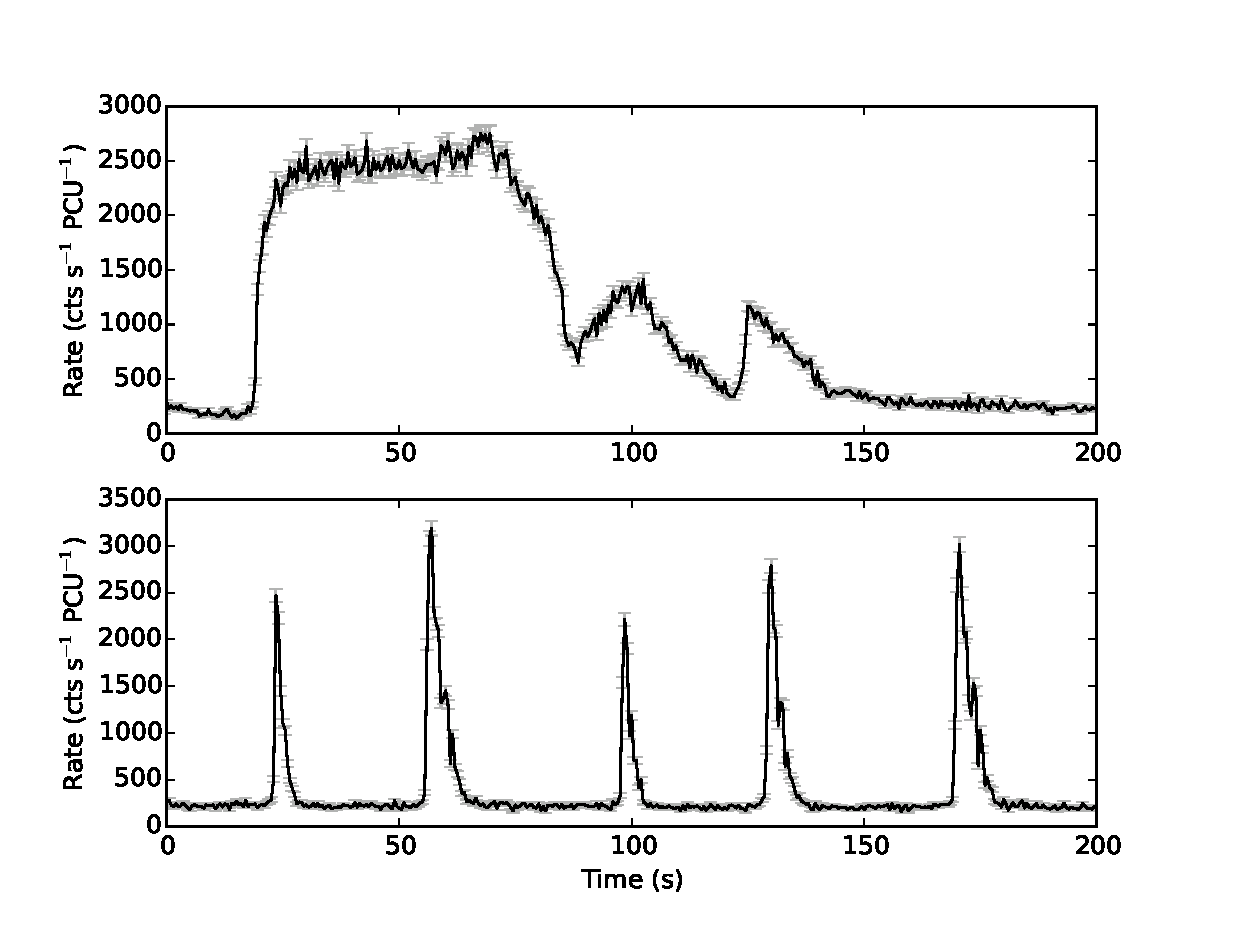
\includegraphics[width=.9\linewidth, trim= 0mm 0mm 0mm 80mm,clip]{images/bagnoli_bursts.eps}
  \caption[An \textit{RXTE}/PCA lightcurve\index{Lightcurve} of the Rapid Burster, showing a number of typical Type II X-ray bursts.]{An \textit{RXTE}/PCA\indexrxte\indexpca\ lightcurve of MXB 1730-335 (also known at the `Rapid Burster', showing a number of typical Type II X-ray bursts.}
  \label{fig:BgB}
\end{figure}

\par Type II bursts have definitively been observed in only two objects: the neutron star LMXBs MXB 1730-335\index{Rapid Burster} (also known as the `Rapid Burster', \citealp{Lewin_TypeII}) and GRO J1744-28\index{Bursting Pulsar}\index{GRO J1744-28|see {Bursting Pulsar}} (also known as the `Bursting Pulsar', \citealp{Paciesas_BPDiscovery}).  In both objects, Type II bursts have been observed during the soft state\index{High/Soft state} portion of multiple outbursts; this in turn suggests that the ability to produce Type II bursts is a property of the system, rather than the property of a specific outburst\index{Outburst}.  There have been claims of Type II-burst-like features during outbursts of a number of other LMXBs, such as SMC X-1\index{SMC X-1} \citep{Angelini_SMC}, but whether these features are the same phenomenon remains unclear.
\par The Rapid Burster\index{Rapid Burster} is an LMXB located in the globular cluster Liller 1\index{Liller 1} \citep{Lewin_TypeII}.  No pulsations\index{Pulsar} have been detected from the system, and as such the spin\index{Spin} of its compact object\index{Compact object} is not known.  However, the presence of Type I\index{X-ray burst!Type I} bursts from this object confirms that the compact object is a neutron star \citep{Hoffman_RB}.  Due to its location in a globular cluster, a number of infrared sources are consistent with the X-ray position of the Rapid Burster, and it is unclear which, if any, is the companion star\index{Companion star} in the system \citep{Homer_RBNoSec}.  However, also due to its association with Liller 1, the distance to the Rapid Burster is known to be 8.9--10\,kpc \citep{Ortolani_LillerD}.  Using this information, it has been shown that the persistent emission\index{Persistent emission} from the object during outburst peaks at no more than 20\% of its Eddington Limit\index{Eddington limit} \citep{Bagnoli_RB}.  The X-ray luminosity of the system at the peak of a Type II burst is around 100\% of its Eddington Limit \citep{Tan_RBBursts,Bagnoli_PopStudy}.  In addition to Type I and Type II bursts, variability\index{Variability} has been observed in the Rapid Burster which is remarkably similar to that associated with GRS 1915 and IGR J17091\index{GRS 1915+105}\index{IGR J17091-3624} (see Section \ref{sec:1915}), suggesting a possible link between these types of variability.
\par The Bursting Pulsar\index{Bursting Pulsar} is an LMXB located in a region of the sky very close to the Galactic centre.  Although Type I\index{X-ray burst!Type I} bursts have not been observed from this system, a coherent 2.14\,Hz X-ray pulsation seen from the object proves that the compact object\index{Compact object} is a pulsar\index{Pulsar} \citep{Kouveliotou_BPPulse} and hence a neutron star.  The distance to the object is $\sim3.4$--4.1\,kpc \citep{Sanna_BP}, and the nature of the companion star\index{Companion star} is unknown.  The persistent emission\index{Persistent emission} from the Bursting Pulsar is believed to peak at $\sim100$\% of its Eddington limit during outbursts, while its peak luminosity during Type II bursts greatly exceeds the Eddington limit\index{Eddington limit} \citep{Sturner_BPNature}.

\subsection{A History of Models of Type II Bursts}

\label{sec:TIImod}

\par \index{X-ray burst!Type II}No models have been proposed which can fully explain Type II bursting behaviour, but several models have been proposed in the context of Type II bursting from the Rapid Burster MXB 1730-33\index{Rapid Burster}.  A number of models invoke viscous instabilities\index{Instability} in the inner disk\index{Accretion disk} as the source of cyclical bursting: for a more detailed review of these models, see \citet{Lewin_Bursts}.
\par One such model was presented by \citet{Taam_Evo}.  They show that a disk\index{Accretion disk} that would be expected to be unstable due to the instability\index{Instability} described by \citealp{Shakura_Instab} can be stabilised by non-local energy transfer.  However they find that this effect is not sufficient to stabilise a disk in the case where viscous stress in the disk scales with local pressure.  In this case, they instead find that a limit cycles of behaviour can be set up, resulting in quasiperiodic flaring which the authors argue is similar to that seen in the Rapid Burster\index{Rapid Burster}.
\par \citet{Walker_Type2Mod} suggests that, for a neutron star\index{Neutron star} with a radius less than its ISCO\index{Innermost stable circular orbit}, a similar cycle of accretion\index{Accretion} can be set up when considering the effects of a high radiative torque.  In their scenario, \citeauthor{Walker_Type2Mod} find that pressure in the inner accretion disk\index{Accretion disk} of such an ultra-compact neutron star is entirely dominated by radiation stresses.  This leads to an unstable and highly non-linear region of the disk, leading to strong aperiodic variability.
\par \citet{Spruit_Type2Mod} (see also \citealp{Dangelo_Episodic1,Dangelo_Episodic2}) use a different approach.  Their model shows that, in some circumstances near the boundary of the propeller regime\index{Propeller effect}, the interaction between an accretion disk\index{Accretion disk} and a rapidly rotating magnetospheric boundary\index{Magnetospheric radius} can naturally set up a cycle of discrete accretion\index{Accretion} events rather than a continuous flow (for a description of this instability in a more general context, see Section \ref{sec:hic}\index{Hiccup accretion}).  The authors specifically discuss this flaring in the context of the Rapid Burster, noting a number of similarities between the output of their models and the properties of flares seen from the Rapid Burster.  However, they note a number of key ways in which their model differs from observations: the flares produced by their model are strictly periodic for a given accretion rate, and consequently the observed relationship between burst waiting time and burst fluence in the Rapid Burster cannot be reproduced.
\par In Chapter \ref{ch:BPbig} I perform a population study\index{Population study} of bursts from the Rapid Burster-like\index{Rapid Burster}\index{Bursting Pulsar} Bursting Pulsar, and use my results to better evaluate the models proposed to explain the Rapid Burster.  In Chapter \ref{ch:BPletter} I also consider an instability\index{Instability} similar to that proposed by \citet{Spruit_Type2Mod} to explain a previously undiscovered variability\index{Variability} during the late stages of outbursts from thr Bursting Pulsar.